 

\begin{quotation}
  To understand brain function, the focus of [our] investigations must
  expand from detailed responses and structure of single cells to
  include unit responses to the activity of other cells, and how these
  responses are distributed over a population of similar cells as
  wells as across populations of different cells.  - \emph{\citet{Shamma:1998}}
\end{quotation}



% =========================================================================

\section{Introduction}

Shihab Shamma calls upon the science community, particularly members
of its physiology and neuroscience subgroups, to investigate the role
of populations of neurons in to pay attention to the role of
populations of neurons in neurophysiology. In this chapter I intend to
draw on the wealth of experimental data accumulated by the auditory
neuroscience community to create a detailed, biophysically-realistic
neural network model of the cochlear nucleus stellate network.  The
design and methods for the construction of the model will provide
insights relevant to other neural network models, especially those
that use highly-specific sensory pathways.

\medskip{}

Though it remains the case that ``choices, assumptions, and guesses
(are) an integral part of neuronal modeling''
\citep{SegevBurkeEtAl:1998}, there is much to be gained from
biophysically-realistic modeling approaches, especially in the heavily
experimented cochlear nucleus. The developments in computational power
and enhanced experimental techniques in multi-unit recordings are
enabling more detailed neural models. Examples of parameter estimation
and fitting in neural models are also becoming more advanced, for
example NeuroFitter \citep{citation} and MultiRunFitter (a feature in
NEURON).  \yellownote{See further on neural detail in auditory system
  \citep{LuRubioEtAl:2008}}

\medskip{}

\yellownote{Discuss use of Poisson models vs HH-like models.  Discuss
  single cell simulation vs whole network simulation during
  optimisation.}  To develop and optimise detailed neural models and
neural network models, reproducible research methods are required. In
this chapter we use a tabular method, introduced by
\citet{NordlieGewaltigEtAl:2009}, to summarise the neural models used in each
optimisation step. This method aims to show a consistent and
recognisable format for presenting various neural network models and
their constituents.  The tables consist of A) the model summary, B)
cell type populations, C) connectivity between cell types, D) neuron
and synapse models, and E) optimisation parameters.

\medskip{}

In this chapter, I construct the stellate network of the cochlear
nucleus (Fig.~\ref{fig:microcircuit}) using a sequential method.  The parameters of each cell type
are fixed based on experimental data or are optimised based solely on
responses to simple stimuli.  Each cell type is shown with its excitatory-inhibitory responses area (EIRA) and PSTH (although this may vary within cell type). Golgi cells (G) receive a range of fibres centred on BF
The stellate network model drawn in Fig.~\ref{fig:microcircuit} describes the following
cells and models:
\begin{enumerate}
\item the Carney phenomenological auditory model
  \citet{ZilanyBruceEtAl:2009}: This model provides spiking input to
  cochlear nucleus neurons across frequencies and spontaneous rate
  types of the auditory nerve from an arbitrary input stimulus. The
  base line in Fig.~\ref{fig:microcircuit} is a simplification of
  auditory nerve fibres (ANF) from low best frequency (BF) to high BF
  (left to right). The model reproduces responses for high and low SR
  ANFs at 100 sections across the frequency range.
\item the Golgi cell: a GABAergic VCN marginal shell unit that is
  presumed to regulate excitability in the granule cell domain and
  core VCN units \citep{FerragamoGoldingEtAl:1998}. The only \emph{in vivo} study shows a type I/III response area and PSTHs with unusual or chopper characteristics in marginal shell units\citep{GhoshalKim:1997}. 
\item the D-stellate cell: the glycinergic, large multipolar cell with
  onset-chopper PSTH response acts as a coincidence detector. Its
  large dendritic area increases its response to noise allowing it to
  behave as a wide-band inhibitor in the VCN, DCN, and contralateral CN 
  \citep{SmithMassieEtAl:2005,ArnottWallaceEtAl:2004,NeedhamPaolini:2007}.
\item the Tuberculoventral cell: a glycinergic, type-II EIRA unit in
  the deep layer of the DCN \citep{SpirouDavisEtAl:1999}.  This cell acts as a delayed
  echo-suppressor and narrow-band inhibitor, with recurrent
  connections between D- and T-stellate cells in the VCN \citep{Alibardi:2006,OertelWickesberg:1993,WickesbergWhitlonEtAl:1991}; and 
\item the T-stellate cell: one of the major output projection cells of
  the cochlear nucleus to the inferior colliculus, this multipolar
  neuron has been shown to have robust spectral representation and
  enhanced synchronisation to modulation in speech sounds \citep{BlackburnSachs:1990,KeilsonRichardsEtAl:1997}.
\end{enumerate}

\begin{figure}[htb]
  \centering
  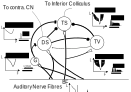
\includegraphics[width=\textwidth]{gfx/CNcircuit}
  \caption{Cochlear nucleus stellate microcircuit (see text for details). }
  \label{fig:microcircuit}
\end{figure}


\medskip{}

Detailed model requires a good input model, a good neural model and
experimental data with which to fit the parameters.  \yellownote{In
  this para: Connect the introduction section to the Auditory model
  below. Discuss the use of the Carney model in the CN stellate
  model.}


\section{Auditory Model}



Advanced auditory fidelity and localisation is an exceptional feature
of hearing perception in animals, despite the input at the
round-window of the cochlea being one-dimensional.  Modelling in the
auditory periphery has benefited extensively from the work of
Liberman, Greenwood, Patterson, Young, Sachs and others, in acoustic
\texttt{in vivo} experiments. The methods of modeling in the auditory
system over the last 30 years have expanded our understanding of the
mechanical processes in the middle ear and cochleae, and specialised
synapse between the inner hair cell and the auditory nerve
\citep{DavisVoigt:1991,Carney:1993,MeddisHewittEtAl:1990}.


To understand the auditory system, one must first understand the
processes in which sound enters the ear and is then transformed to
neural signals in the auditory nerve. Mechanical vibrations at the
eardrum (tympanum) are conducted by the middle ear bones to vibrations
in the inner ear (cochlea). They are then transformed to chemical
signals in the inner hair cells and then to electrical potentials of
the auditory nerve fibres. This processing enters a bottle-neck at the
auditory nerve, where a group of highly specialised heterogeneous
neurons in the cochelar nucleus process the incoming information in
several pathways including temporal, spectral, onset and
other feature-based information pathways.

\medskip{}

The auditory system is topographically ordered from the basilar
membrane to the cortex in terms of frequency selectivity, also called
tonotopicity \citep{YoungOertel:2004}.  The population of auditory
nerve fibres (ANFs, Fig.~\ref{fig:CNdiagram}), bifurcate after
entering the cochlear nucleus to innervate the VCN and DCN\@,
retaining their tonotopic order
\citep{Lorente:1981, Liberman:1982, Liberman:1993}. Type 1 ANFs are
categorised into high spontaneous rate (HSR) and low spontaneous rate
(LSR) fibres \citep{Liberman:1978}, where LSR fibres have a higher
threshold and wider dynamic range than HSR fibres. They also project
to the granule cell domain (GCD)
\citep{RyugoParks:2003, RyugoHaenggeliEtAl:2003} along with the
smaller, unmyelinated type 2 ANFs, which suggests they play a
different role in sound processing to HSR fibres.

\medskip{}

\begin{figure}[tbh]
  \begin{center}
%    \includegraphics[keepaspectratio=true]{NoFigure}
    \resizebox{2.25in}{!}{\includegraphics[width=2.25in,keepaspectratio]{gfx/Cat_Human_CN}}
    \caption{Cochlear nucleus innervation in Man and Cat. \citep[find out which publication printed this!][needs permission]{RyugoParks:2003,Ryugo:1992,Spoendlin:1973}}
    \label{fig:CNdiagram}
  \end{center}
\end{figure}


\medskip{}

\yellownote{Discuss auditory model history. Expand reasons for wanting
  to create a biophysically realistic model of the CN\@. Discuss reason
  for using whole network in TV and TS optimisation} 

\medskip{}

\yellownote{a paragraph on the history of AN modelling
  \citep{LeakeSnyderEtAl:1993, ArnesenOsen:1978, CloptonWinfieldEtAl:1974}.
  Perhaps Rose et al 1959 would be better suited here}
%
\medskip{}

In examining the properties of a detailed neural model of the cochlear
nucleus, a realistic and phenomenologically sound auditory model is
needed to represent sounds and transformations that occur in the
central auditory system.


\yellownote{AN model paragraph has been changed} The auditory nerve inputs to
the cochlear nucleus model neurons are provided by phenomenological auditory
periphery models: the ARLO model \citep{HeinzZhangEtAl:2001}; the Bruce model
\citep{BruceSachsEtAl:2003, ZilanyBruce:2006, ZilanyBruce:2007}; and the Zilany
model \citep{ZilanyBruceEtAl:2009}. The AN model consists of an outer/middle ear
pre-processing filter, a cochlea filterbank, IHC-to-AN synapse model and
dead-time modified Poisson spike generator, as shown in
Fig.~\ref{fig:ZilanyBruceFig}. \citep{HeinzZhangEtAl:2001} incorporated cochlea
filters based on the critical bandwidths obtained from psycho\-physical
experiments in humans. The ARLO model of the cat auditory periphery, with
non-linear compression and two-tone suppression, is used in this study except in
the vowel simulation where the human auditory periphery model is used.

\medskip{}

The \citet{ZilanyBruce:2007} model improves the previous AN model by an
additional signal path and its predictions have matched a wide range of
physiological data in normal and impaired cat data. The most recent AN model
comprises an power-law synapse model, with internal $1/f$ noise, that enhances
the behaviour of long-term dependence in ANFs \citep{ZilanyBruceEtAl:2009}.

\medskip{}

\yellownote{Why is it the cat model? updating Carney model?} Updating of the
Carney auditory model has led to the change in the model's configuration from an
original implementation of the rat model.  The default species is the cat and
will be used in the data presented in this chapter.

\begin{figure}[tbh]
  \begin{center}
%    \resizebox{3.5in}{!}{\includegraphics[keepaspectratio=true]{NoFigure}}
    \resizebox{\textwidth}{!}{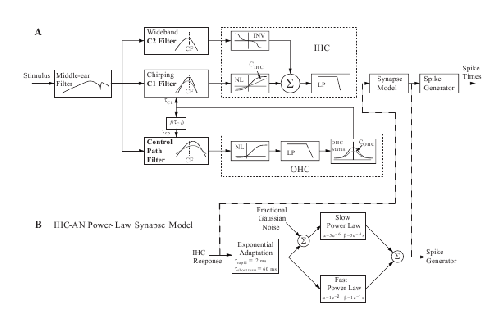
\includegraphics[keepaspectratio=true]{gfx/ZilanyCarney-JASA-2009-Fig2.eps}}
    \caption{Auditory periphery model with dual power-law synapse \citep[originally printed in ][]{ZilanyBruceEtAl:2009}.}
    \label{fig:ZilanyBruceFig}
  \end{center}
\end{figure}\yellownote{if this figure is used it needs permission by the original authors}


\subsubsection{Physiological Responses}

\yellownote{TODO: serious reworking to be done here}
Analysis of the frequency response area of ANF generates known
parameters for each fibre, these are:
\begin{itemize}
\item the spontaneous rate (SR), generated in silence and is
  categoried into two groups High SR ($>$18 sp/s) and Low SR ($<$ 18
  sp/s);
\item threshold, the sound pressure level(SPL) at which the cell
  responds above the spontaneous rate
\item characteristic frequency (CF)
\end{itemize}

\medskip{}

% \begin{figure}[tbp]
%   \begin{center}
%     \resizebox{3.5in}{!}{\includegraphics[keepaspectratio=true]{NoFigure}}
%     % \resizebox{3.5in}{!}{\includegraphics[keepaspectratio=true]{C:/nrnwork/oldwork/ra/TTCsANLSR}}
%     % \resizebox{3.5in}{!}{\includegraphics[keepaspectratio=true]{C:/nrnwork/oldwork/ra/TTCsANHSR}}
%     \caption{Response areas of low and high spontaneous rate ANFs calculated from the  }
%     \label{fig:CochlearTTCs}
%   \end{center}
% \end{figure}

%% \begin{figure}
%%   \begin{center}
%%     \includegraphics[keepaspectratio=true]{gfx/ClickFB}
%%     \caption{Cochlea Filterbank to click stimuli}
%%     \label{ClickFB}
%%   \end{center}
%% \end{figure}

% \begin{figure}[tbh]
%   \begin{center}
% %    \resizebox{3.5in}{!}{\includegraphics[keepaspectratio=true]{NoFigure}}
% %    \resizebox{3.5in}{!}{\includegraphics[keepaspectratio=true]{ClickDelay}}
%     \caption{Response of AN and CN cells to click stimuli. }
%     \label{fig:ClickDelayAN}
%   \end{center}
% \end{figure}


\section{Cochlear Nucleus Stellate microcircuit}

\subsection{Neural models}

[Discuss R\&M model]
\yellownote{TODO: Is this a replication of other work or have I changed it enough that it needs to be shown or too general to go in this chapter (put in Methods Chapter}

\medskip{}

\subsection{Tonotopic connectivity}

The channels are separated using even spatial distance (based on the
basilar membrane and auditory nerve separation) with centre frequency
calculated by the Greenwood function for the cat
\citep{Greenwood:1990}. \yellownote{More detail in Appendix}

\medskip{}

Figure~\ref{fig:CNconn} shows the method for Gaussian spread of
connections between cell types in the CN\@.  The channels are separated
using even spatial distance used for the AN filterbank.


\begin{figure}[tbh]
  \begin{center}
%    \resizebox{3.5in}{!}{\includegraphics[keepaspectratio=true]{NoFigure}}
    \resizebox{\textwidth}{!}{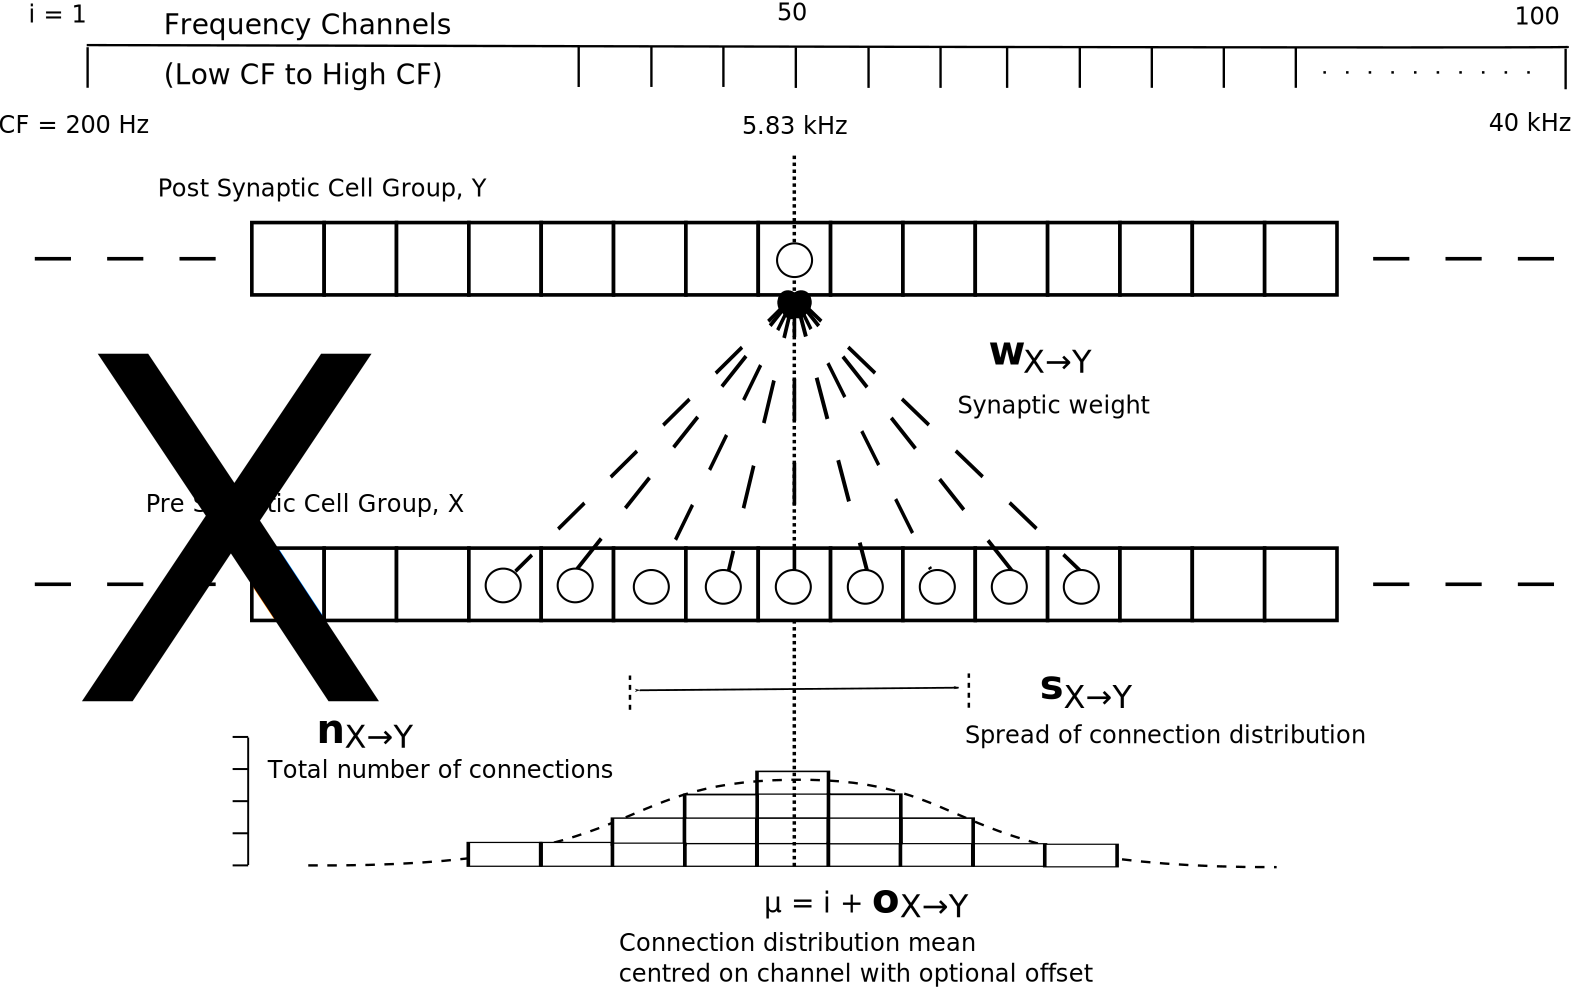
\includegraphics[keepaspectratio=true]{gfx/CNConn}}
%    \resizebox{0.8\textwidth}{!}{\input{./gfx/CNConn.tex}}
    \caption{Gaussian connection between cell types in cochlear
      nucleus. }
    \label{fig:CNconn}
  \end{center}
\end{figure}






%%% Local Variables: 
%%% mode: latex
%%% mode: tex-fold
%%% TeX-master: "SimpleResponses"
%%% TeX-PDF-mode: nil
%%% End: 
